\documentclass[onecolumn, draftclsnofoot,10pt, compsoc]{IEEEtran}
\usepackage[utf8]{inputenc}
\usepackage{graphicx}
\graphicspath{ {./} }
\usepackage{caption}
\usepackage{url}
\usepackage{setspace}
%\usepackage{parskip}
\usepackage{longtable}
\usepackage{hyperref}
\hypersetup{
    colorlinks=true,
    linkcolor=blue,
    filecolor=magenta,      
    urlcolor=blue,
}

\usepackage{geometry}
\geometry{textheight=9.5in, textwidth=7in}

% 1. Fill in these details
\title{Group 73: Progress Update}
\author{Stephen Hoffmann, Stewart Rodger, Nicholas Pugliese, Kyle Tyler, Symon Ramos}
\date{February 2019}
\def \CapstoneTeamName{		    Group 73: VR Press}
\def \CapstoneTeamNumber{		73}
\def \GroupMemberOne{			Symon Ramos}
\def \GroupMemberTwo{			Stephen Hoffman}
\def \GroupMemberThree{			Nicholas Pugliese}
\def \GroupMemberFour{			Stewart Rodger}
\def \GroupMemberFive{			Kyle Tyler}
\def \CapstoneProjectName{		Developing Virtual Reality Based Training Experiences for HP's PageWide Web Press Product Line}
\def \CapstoneSponsorCompany{	HP Inc}
\def \CapstoneSponsorPerson{		Tim Holt}



% 2. Uncomment the appropriate line below so that the document type works
\def \DocType{		
				Design Document
				%Progress Report
				}
			
\newcommand{\NameSigPair}[1]{\par
\makebox[2.75in][r]{#1} \hfil 	\makebox[3.25in]{\makebox[2.25in]{\hrulefill} \hfill		\makebox[.75in]{\hrulefill}}
\par\vspace{-12pt} \textit{\tiny\noindent
\makebox[2.75in]{} \hfil		\makebox[3.25in]{\makebox[2.25in][r]{Signature} \hfill	\makebox[.75in][r]{Date}}}}
% 3. If the document is not to be signed, uncomment the RENEWcommand below
%\renewcommand{\NameSigPair}[1]{#1}

%%%%%%%%%%%%%%%%%%%%%%%%%%%%%%%%%%%%%%%
\begin{document}
\maketitle
    \begin{abstract}
    % Copied from group problem statement
   Virtual reality (VR) training simulations provide the opportunity to implement an interactive learning experience that improves on traditional learning methodologies. We propose a series of VR-based training scenarios designed to train personnel on how to operate machinery from HP’s PageWide Web Press product line. Developing these training scenarios will improve the effectiveness of HP’s current training procedure as well as mitigate the costs and risks of handling real machinery by the trainees. Using the Unreal engine, the Datasmith CAD model importer, and HP's Microsoft Mixed Reality headset we will build a program to solve the inefficient training problem. Data recording of user actions will be collected to measure and justify the simulation’s effectiveness. By integrating VR training simulations into the current training procedure, we enable the training process to be more effective while at the same time adding incentive for HP to further pursue VR training-related development. This program we create will serve as a feasibility prototype to show to HP that a virtual reality program is a viable alternative to their current training program.
    \end{abstract}
\newpage
\pagenumbering{arabic}
\tableofcontents
% 7. uncomment this (if applicable). Consider adding a page break.
%\listoffigures
%\listoftables
\clearpage

%For the report, the document will:

%briefly recap the project purposes and goals
%describe where you are currently on the project
%describe what you have left to do
%describe any problems that have impeded your progress, with any %solutions you have
%include particularly interesting pieces of code (if coding is %involved)
%(research only) include descriptions of preliminary results
%(interface design only) include description of first user study, %hopefully with results
%include images of your project -- screen shots, photos, whatever is %appropriate
%at least alpha level functionality should be in evidence at the %draft turn-in (end of week 6), with beta level functionality at the %final submission (end of term).

% 8. now you write!
\section{Recap of Project Purposes and Goals}

The goal of this project is to demonstrate the feasibility of creating and using a Virtual Reality (VR) training program for HP Inc.'s industrial printer: the HP Page-Wide WebPress. When a customer purchases a Page-Wide WebPress, they must be flown out to an HP location that houses a WebPress to attend an intensive, week-long training seminar. This training program is not only time-consuming, but very expensive. This project aims to create a prototype VR training program to showcase the feasibility of replacing at least one of the in-person seminar days with a virtual reality program that can be shipped (a long with a VR headset) to the customer's location.

This feasibility prototype will include two different modes of operation: "scenario mode" and "sandbox mode." Scenario mode will provide reenactments of WebPress training modules from the seminar training material (for example, replacing a print cartridge). Sandbox mode will not be restricted to single scenario modes and will allow the user to interact with any part of the WebPress they wish in a convincing virtual environment.

\section{Current State of Project}

First and foremost: the alpha release as described in this document may be viewed at this link: 

\noindent
\href{https://github.com/SilverGekko/cs461}{https://github.com/SilverGekko/cs461}\\

\noindent
Our team has been able to construct the entire virtual environment inside of a 3D model of a warehouse. Models we have added include the Web Press printer itself (modeled after the T240 model), ink barrels, computers, desks, chairs, an office space to serve as our tutorial room, lights, E-Stop buttons, spare printheads, tables, cabinets, and cautionary tape. The Web Press printer is comprised of multiple models, including the printer itself, the winder and unwinder (which is where the paper is fed in and out respectively), and individual printheads of different colors. The models are semi low-poly (which means that its quality isn't incredibly detailed) and designed to be believable and cohesive to the narrative while also being inexpensive to create. We have also implemented basic functionality with the buttons on the Web Press and the ability to toggle lights on the printer. We have also added a main menu feature. In addition, we have also been developing a user interface heads-up display (HUD) that will provide the user with information when wearing the headset. With this and the environment at our disposable, we will be capable of moving forward with the next phase of our project development for this term. 

\begin{figure}[ht!]
    \centering
    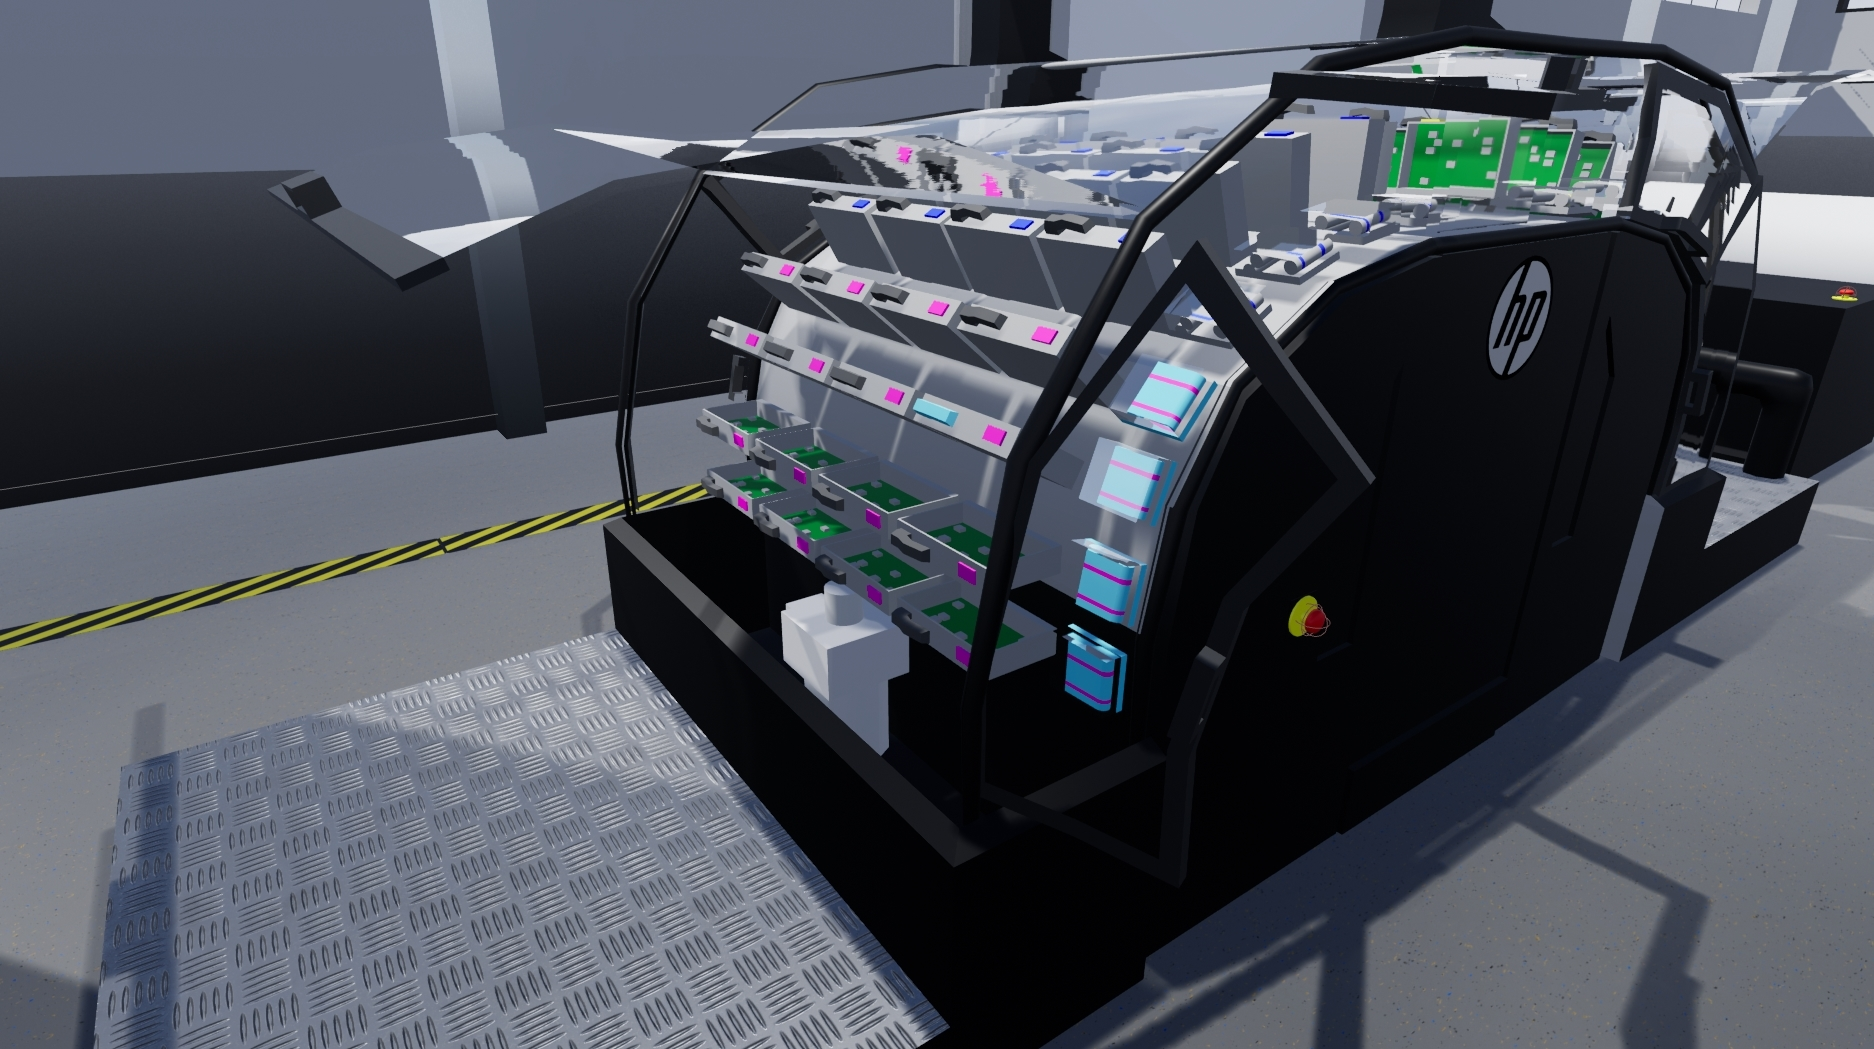
\includegraphics[width=0.85\textwidth]{press1.png}
    \caption{Web Press Printer 3D Model}
    \label{fig:printerModel}
\end{figure}

Our current objective is to implement a training module that can simulate a procedure that is currently being taught to users. Our team has investigated several T2XX Web Press documents, including the T2XX Web Press Operating Manual, the Preventative Maintenance Manual 2177, and the T2XX Web Press Documentation and Training Documents. The most promising procedure that we encountered was the replacement of printheads. A common procedure, the T2XX Web Press Operating Manual outlines a sequential series of steps that the user has to complete in order to successfully remove the existing printhead and insert the new one. In a later section detailing common troubleshooting scenarios, several scenarios where the replacement of printheads would be applicable are included, such as when a printhead is overheating. The figure below outlines the user workflow of the replacement of printheads. Note that one suggestion that our client had was to add references to the sections in the manual from which each step replicates. By doing so, we could have a more justifiable basis to present our training module to individuals who conduct the current training classes for those learning how to use the Web Press.

\begin{figure}[ht!]
    \centering
    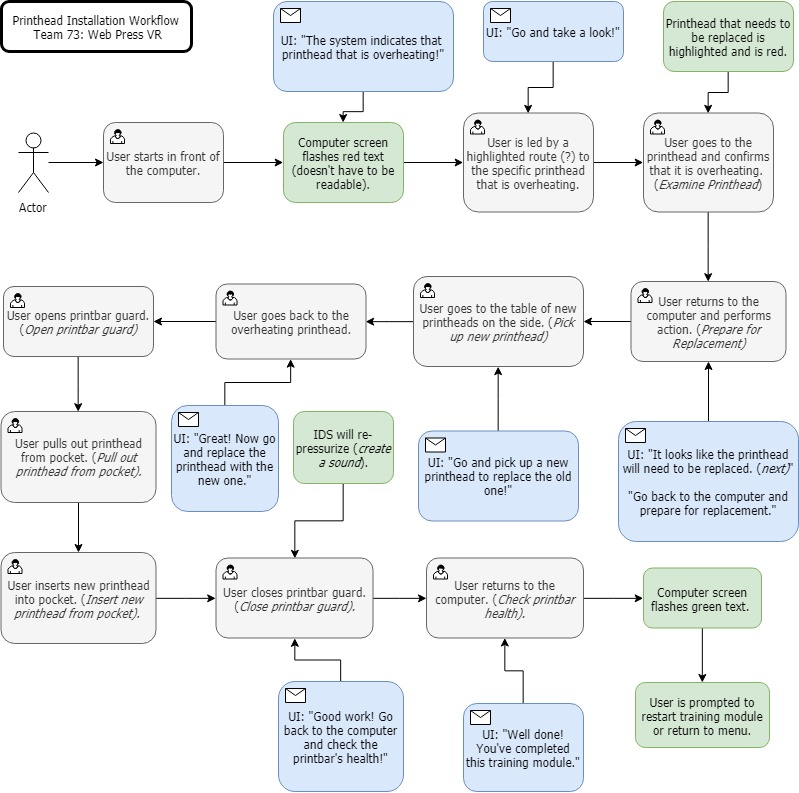
\includegraphics[width=0.85\textwidth]{PrintheadInstallationWorkflow.jpg}
    \caption{The Printhead Installation Workflow}
    \label{fig:workflow}
\end{figure}

Logistically, our team has met multiple times with our client to discuss the current state of our project. These meetings have all gone well and are valuable in giving us direction for the next steps we are going to take. We have also participated in a workshop to practice our elevator pitches with other students. Having the ability to discuss our project with the right amount of detail depending on our audience is crucial to being able to convey the significance of our project. In addition, we've also met with Kirsten and another capstone team to evaluate the draft of our poster board for the expo. We found many improvements that we could implement in order to have a better expo experience. We've also met many times as a team to discuss project objectives, implement models and features to the virtual environment, and program in small groups. Because of the size of our team and differences in schedules, we aren't all always able to regularly meet. This, however, works to our advantage, as having small groups of 2-3 meet every often enables us to have more focus on our assigned objectives. 

\subsection{Tutorial Overview}

Our client has emphasized that this program will eventually be used by actual web press operator trainees. These trainees may have never used Virtual Reality before, and thus will probably need dedicated tutorials to learn how to use the Virtual Hardware tutorial. Our team decided on three main tutorials to illustrate the basic skills needed to use a Virtual Reality program:

\begin{itemize}
    \item Looking around the room in VR ("Seeing" tutorial)
    \item Using the hand-held controllers to teleport ("Moving" tutorial)
    \item Picking up objects and pressing buttons ("Interacting" tutorial)
\end{itemize}

Each of these tutorials takes places in a section of the environment designed to look like an office cubicle. This tutorial space takes place in a separate level than the Web Press itself. The user may leave this tutorial level and go to the main Web Press level by clicking a button on the user interface. The tutorial instructs the user to do this once the three tutorials listed above are done, but an experienced user may exit the tutorial at any time by accessing the same menu.

\subsubsection{Seeing Tutorial}

The seeing tutorial teaches the user that they may look around with full 3D motion while wearing the headset. The tutorial is completed by making the user point to an onscreen crosshair at a computer monitor on a desk. This process is repeated on three total monitors ranging from in front of the user, to almost directly behind them. The idea is to force the user to physically turn their body around so they learn the extent of the control they have over the viewport with the headset.



\subsubsection{Moving Tutorial}
The moving tutorial teaches the user that they can move around the virtual space by pressing a button on the controller, pointing, and releasing to teleport to that location. The tutorial is completed when the user teleports away from the starting position. This teaches the user how to move around the environment, which they will need to do to complete the training scenarios.   

\subsubsection{Interacting Tutorial}

The interacting tutorial teaches the user that there are objects in the virtual environment that may be interacted with using the handheld controllers by moving the controller over the object in the virtual space and holding down the trigger button. All of the objects in the virtual space that may be grabbed like this are colored the same sky blue color as shown in figure \ref{fig:skyblue}.

\begin{figure}[ht!]
    \centering
    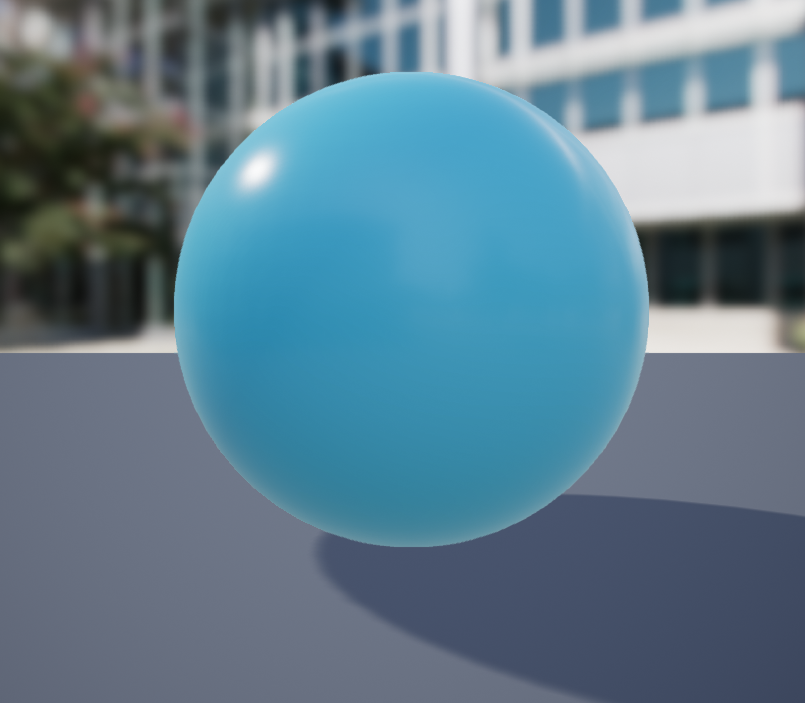
\includegraphics[scale=0.5]{touchMeBlue.png}
    \caption{The specific shade of blue that informs the user they may pick up and manipulate the object.}
    \label{fig:skyblue}
\end{figure}

In addition to learning about "grab me blue," the user will also learn how to press buttons that correspond to the emergency stop buttons location on the Web Press. These buttons are an important part of the operation of the Web Press, so using them as an introduction to intractability will link the users understanding of the tutorial to the actual training scenario in the main level.

\section{Problems and Proposed Solutions}
One aspect of our performance metric for this project is the evaluation and feedback of what would be the audience for our training modules to prove that our methodology of VR training has more merit than the current work procedure. In order to evaluate our project’s effectiveness, our team has determined to utilize System Usability Scale (SUS) forms of which participants who demo our project will be able to fill out anonymously. By gathering this data, we can determine the effectiveness of our method of training as well as note any modifications that could be made in future implementations. Nick has spoken with his team at HP, who have expressed interest in demoing the project, and they would all be great candidates to rate and critique the experience we have created. 


One item that our client specified is designing our project to also adhere to an audience that isn’t well-versed with Virtual Reality. While we are primarily catering to an audience with a technical background, we still have to account for the fact that many who attempt our training module might not be familiar with the use of VR and will require more extensive learning of how to interact with the environment than others. We have thus designed multiple features to account for this: we have implemented a tutorial mode (created in the office space of our environment) in which the user will be tasked with performing basic actions in a cohesive narrative. In this tutorial space, the user are asked to look around, focus their screen towards something, move around, grab items, and interact with the environment. All users are given the option of going through the tutorial mode before attempting the training module. In addition, we have also created an infographic of the Windows Mixed Reality controllers to outline the control scheme, as shown in figure \ref{fig:controllers}. We plan to incorporate this infographic within the Virtual Reality environment itself. 

\begin{figure}[ht!]
    \centering
    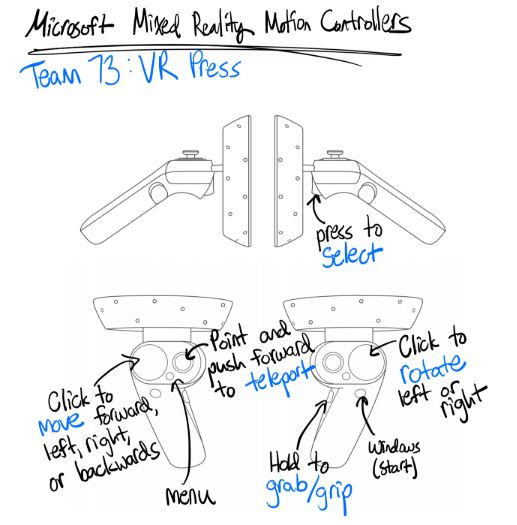
\includegraphics[width=0.85\textwidth]{VRPressInfographic.JPG}
    \caption{Windows Mixed Reality Controller Scheme}
    \label{fig:controllers}
\end{figure}



\newpage
\section{Interesting Code}

\subsection{Blueprints}

We are relying heavily on the visual scripting language unreal provides called "blueprints." They are called blueprints because you create them once, potentially link them to a mesh actor (an object in the game), and then instantiate them into the game world to have an effect.

One such example of a non-trivial blueprint is the one we have made for picking up a printhead out of the WebPress and replacing it back in the exact same spot. This was tricky because we didn't want the user to need pixel-perfect accuracy to have the printhead snap back to its location, so we used some basic vector math to calculate the distance between the starting location and the current location, and then have the object snap back to the starting location if the distance was less than 100 units.

\begin{figure}[ht!]
    \centering
    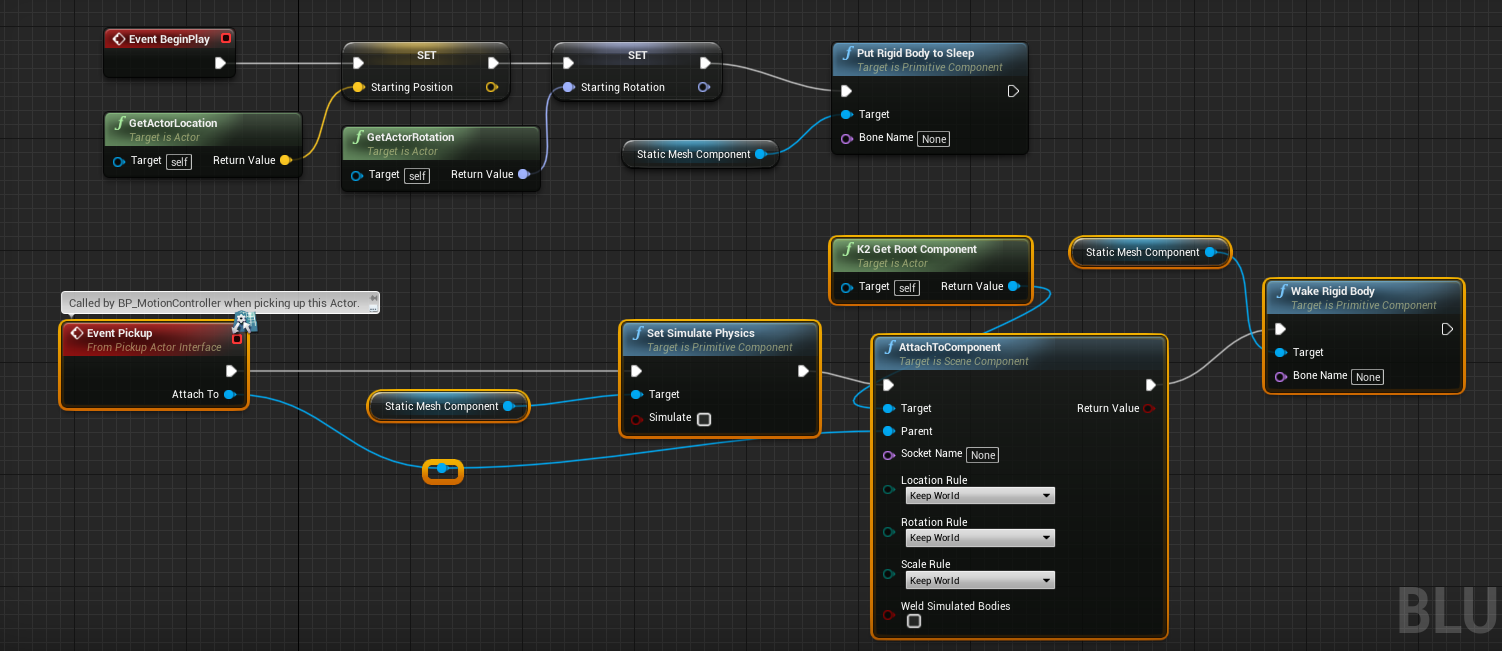
\includegraphics[scale=0.4]{pickup_bp1.png}
    \caption{Pickup event for the replaceable object blueprint. Note the specific activation of the physics for the object once it it removed from its starting location.}
    \label{fig:pickup1}
\end{figure}

\begin{figure}[ht!]
    \centering
    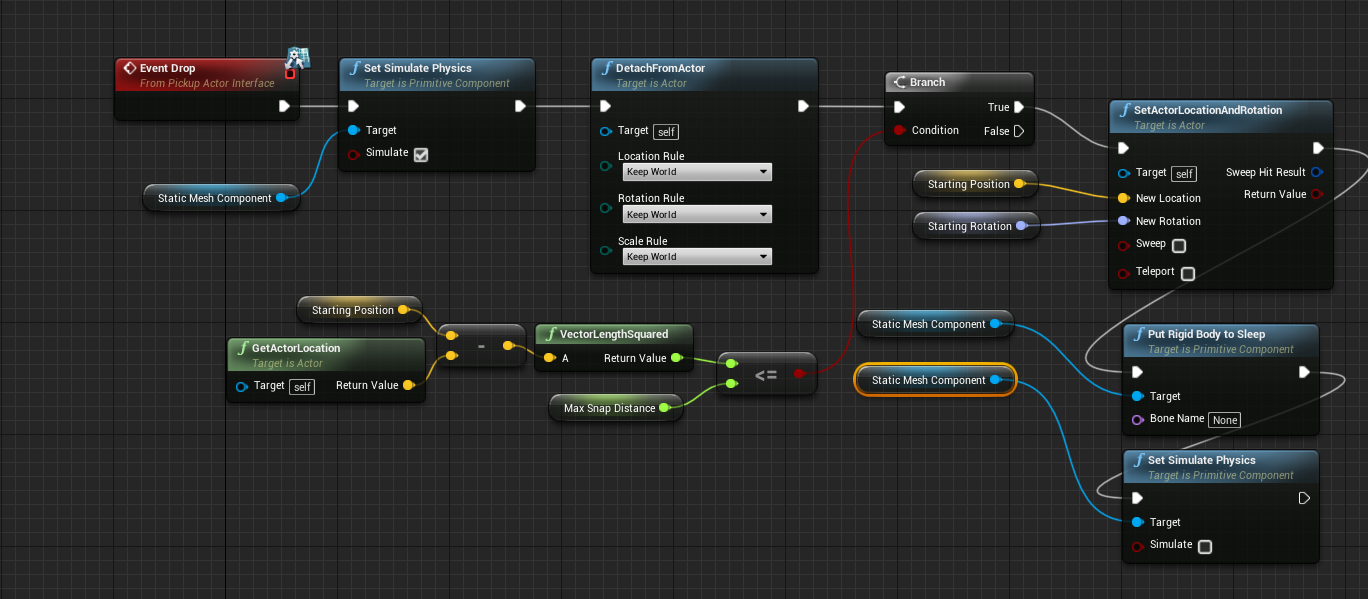
\includegraphics[scale=0.4]{pickup_bp2.png}
    \caption{Drop event for the replaceable object blueprint. Note that if the object is dropped and it is within a specific distance of the starting position, it will snap back to that location and turn off physics again. Else, it will simply drop to the floor with the physics still enabled.}
    \label{fig:pickup2}
\end{figure}

\newpage

The other interesting blueprint we have for this project is the tutorial data flow logic, as seen in Figure \ref{fig:tutorial1}. We plan on following this basic data structure going forward for the scenario:
\begin{itemize}
    \item User has UI prompt (and voiceover) instructing them on what to do next.
    \item If they complete the objective, mark it as done and move on to the next task.
    \item Repeat until scenario ends.
\end{itemize}

Once we turn this into a template, we will have covered what we set out to achieve for this project: to create a tool for HP to expand upon and use for making training scenarios for the WebPress. Stretch goals for the project will be to create more of these scenarios for HP to use and see the value of.

\begin{figure}
    \centering
    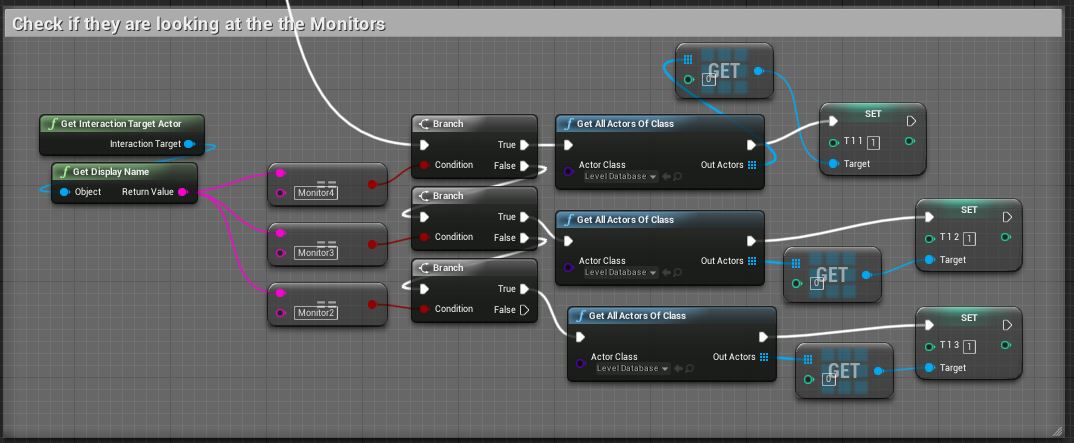
\includegraphics[scale=0.55]{looking_tutorial.png}
    \caption{Data flow for the "looking" tutorial.}
    \label{fig:tutorial1}
\end{figure}

\section{Retrospective: a Week by Week Summary}

The following outlines what we have done during each week of this term. We describe what good happened that week, what changes need to be implemented, and what actions will be implemented to create the necessary changes.

\begin{longtable}{ |p{2cm}||p{5cm}|p{5cm}|p{5cm}|  }
 \hline
 \multicolumn{4}{|c|}{\textbf{Winter Term Retrospective}} \\
 \hline
 \textbf{Week} & \textbf{Positives} & \textbf{Deltas} & \textbf{Actions}\\
 \hline
  % Week one
 1 & 
    Starting week. Requested hardware from McGrath and asked our client, Tim Holt, to setup weekly meetings to go over progress.
    %column two
    & No reply from Tim this week.
    %column three
    & Started creating a 3D model of the WebPress to use in our VR application. Started creating a warehouse environment to serve as the landscape for the program.\\
 \hline
 % Week two
 2 & Our team has brushed up on the unreal engine by going over tutorials for basic level geometry and object placement.
     %column two
    & Basic level landscape created. WebPress mockup added for level blocking. Tim also responsed to our messages and we have set up a recurring meeting.
    %column three
    & Continue working on the 3D models. To do this we went to HP and took reference pictures of the WebPress to use to create our own models, rather than rely on the gigantic CAD files that HP provided us.\\
 \hline
 % Week three
 
 3 & Continuation of last week. Level detail increased, 3D models almost completed.
    %column two
    & This week we sat down with a VR headset and made sure the level geometry actually made sense for an approximately 5-foot 10inch person to walk around in. The scale of the doorways, desks, and objects, as well as the 3D model of the WebPress itself. The user interface was decided upon and development on that was begun. Our client told us he wanted a big focus be on VR tutorials for first time users since the WebPress operators might have no VR experience prior to this training program.
    %column three
    & Wait for the last touches on the 3D models to be done, as well as the first mockup of the user interface.\\
\hline
% Week four
 4 & First steps of a training scenario created. Interactable buttons that change the state of the WebPress with visual clarity.
     %column two
    & The WebPress has "emergency stop buttons" on it that, when pressed, cause the WebPress to completely stop and enter an emergency state where operation will halt until all of the emergency stop buttons in the "pressed" state are switched to the "unpressed" state. We have created an unreal blueprint for these buttons and added dummy functions to the states of the buttons that change a light at the moment.
     %column three
     & 
    Start brainstorming the first scenario we need to create with these stop buttons for next week.\\
\hline
% Week five
 5 & 3D Models of the WebPress fully integrated into the environment. Landscape upgraded to warehouse to serve as a familiar environment.
    %column two
    & The WebPress models have finally been added to the environment! The warehouse environment now includes an office cube space to be used as the tutorial backdrop for the first time VR users.
    
    %column three
    & Keep working on the blueprints for the scenario objects.
    \\
\hline
% Week six
 6 & Brainstormed with client about the training scenario contents. According to our client, if we only implement one training scenario (replacing a printhead on the WebPress) and the sandbox mode that lets the user just play around with the WebPress, we will have completed what he wanted to get out of this senior project.
    %column two
    & We created a workflow diagram (See fig. \ref{fig:workflow}) for how the printhead replacement scenario should go. This information was parsed out of the training manual by one of our team members. We also created a VR controller reference sheet (See fig. \ref{fig:controllers}). A PDF of this sheet will be given to the user outside of the training program so they can get to know the controls. The exact same sheet will also be available for the user to reference inside the VR program (most likely in the form of a poster on the wall) so they do not have to remove their headset to check the controls.
    %column three
    & Keep working on the scenarios now that we have a plan of attack. \\
\hline
% Week seven
 7 & Completed full base tutorial. Started work on the groundwork mechanics for the training scenario.
     %column two
     & Tutorials include introducing the user to using a VR headset by having them look around at fixed points in a room to illustrate full 3D range of motion, introducing the player with the ability to teleport to move around the environment, and showing the user that there are objects (colored with a specific shade of sky blue) the user can pick up and manipulate (coffee cups are used as an example in the tutorial). The user is
     %column three
     & Prepare for alpha release on 2019-02-25. Things still left to be done are fully flesh out the first scenario blueprint by making the different events scripted and flow to each other.\\
\hline
% Week eight
 8 & Alpha release. Groundwork laid down for the scenario (objects such as printheads are now pick up and movable). Remaining task for the scenario: cannibalize the tutorial logic flow and use it for the training scenario.
    %column two
    & Signing up for expo. Poster draft? Peer review
    %column three
    & TBD\\
\hline
% Week nine
 9 & TBD
     %column two
     & TBD
     %column three
     & TBD\\
\hline
% Week ten
 10 & TBD
      %column two
      & TBD
      %column three
      & TBD \\
 \hline
\end{longtable}

\end{document}

